\chapter{Bloemen, vruchten en zaden}\label{ch:g3:flowers-fruits-seeds}

In april staat de kersenboom wit van de bloesem; in juni hangt hij vol
kersen. Waar zijn de \omterm{def:g3:flowers-fruits-seeds:parts}{bloemen} gebleven --- en waar komen de \omterm{prop:g3:flowers-fruits-seeds:transform}{vruchten}
vandaan? Het antwoord is een van de mooiste veranderingen in de levende
wereld: de \omterm{def:g3:flowers-fruits-seeds:parts}{bloem} verdwijnt niet, ze \emph{wordt} de \omterm{prop:g3:flowers-fruits-seeds:transform}{vrucht}.

\section{In een bloem kijken}

\begin{definition}[De delen van een bloem]\label{def:g3:flowers-fruits-seeds:parts}
Een \emph{bloem}\index{bloem} is het deel van de \omterm{def:g1:plants-around-us:plant}{plant} dat de \omterm{prop:g3:flowers-fruits-seeds:transform}{zaden} zal
maken. Van buiten naar binnen:
\begin{enumerate}
  \item de \emph{kroonbladen}\index{kroonblad}, gekleurd en geurend,
        die bezoekende \omterm{prop:g3:sorting-living-things:groups}{insecten} lokken;
  \item de \emph{meeldraden}\index{meeldraad}, dunne stengeltjes
        bestoven met \emph{stuifmeel}\index{stuifmeel}, een fijn geel poeder;
  \item helemaal in het midden de \emph{stamper}\index{stamper}, een
        klein flesje; diep daarin liggen de toekomstige \omterm{prop:g3:flowers-fruits-seeds:transform}{zaden} van de bloem.
\end{enumerate}
\end{definition}

\begin{omfigure}
\begin{tikzpicture}
  \node[anchor=south west, inner sep=0] (img) at (0,0)
    {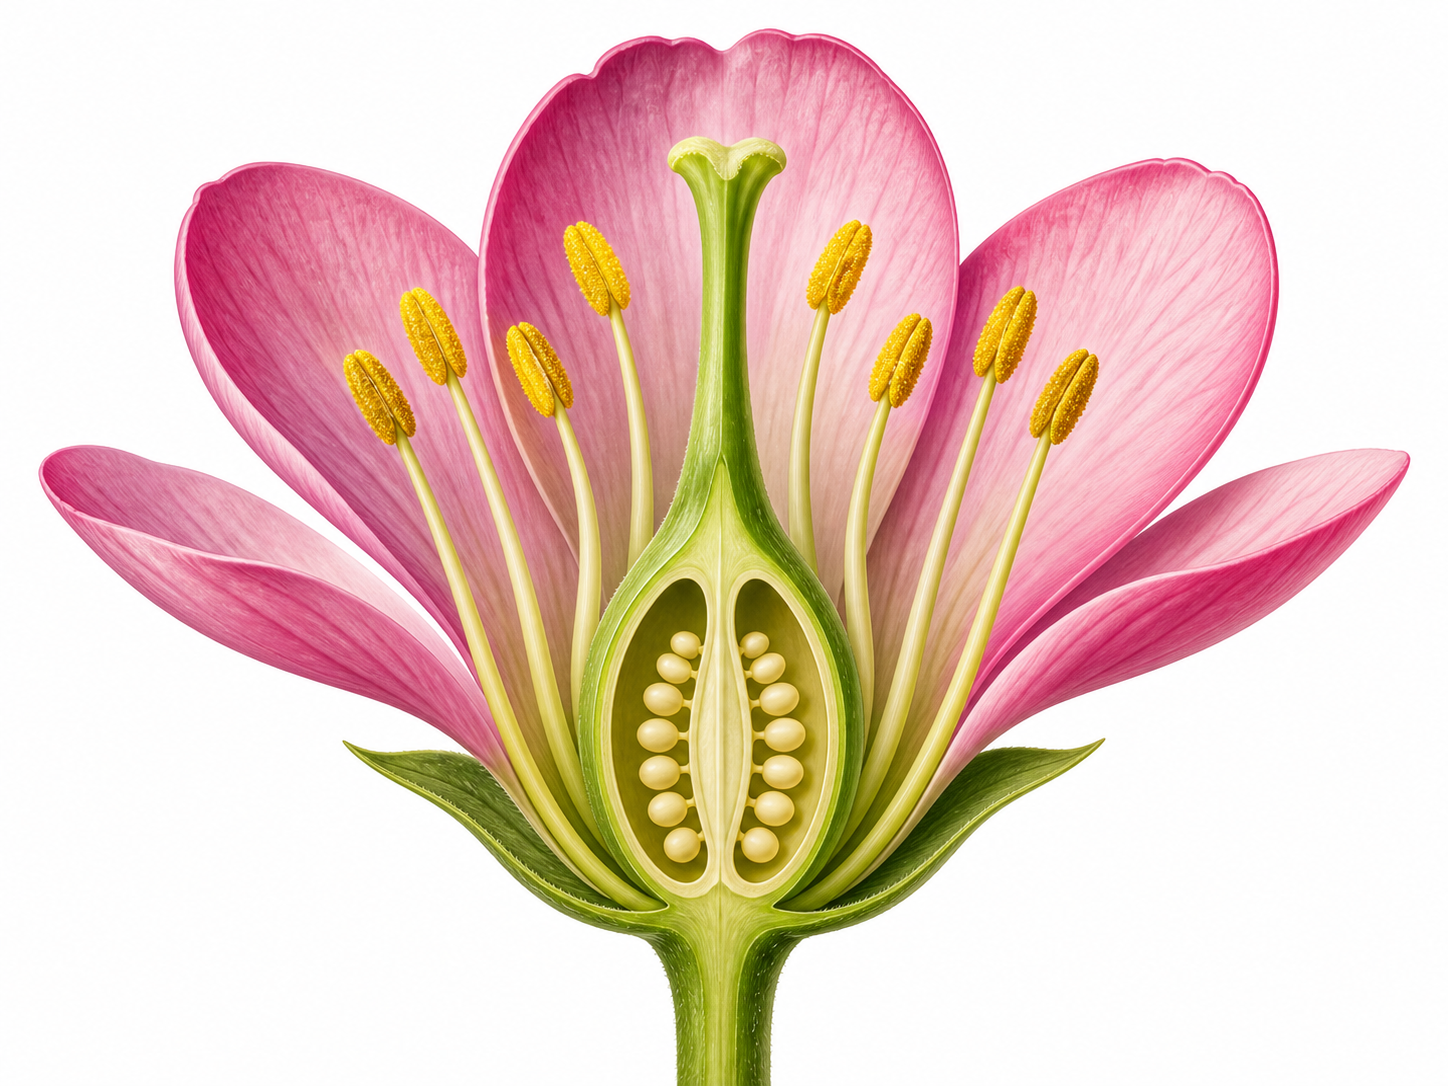
\includegraphics[width=0.6\linewidth]{images/book1/ai/fig-flower-cutaway.png}};
  \begin{scope}[x={(img.south east)}, y={(img.north west)},
      every node/.style={font=\small}]
    \draw[omDef, thick] (0.82,0.80) -- (0.93,0.90) node[above] {kroonblad};
    \draw[omDef, thick] (0.72,0.68) -- (1.03,0.66)
      node[right, align=left] {meeldraad, bestoven\\ met stuifmeel};
    \draw[omDef, thick] (0.56,0.36) -- (1.03,0.34)
      node[right, align=left] {stamper: de toekomstige\\ zaden zitten erin};
    \draw[omDef, thick] (0.505,0.05) -- (0.66,0.04) node[right] {stengel};
  \end{scope}
\end{tikzpicture}

{\small In een doormidden gesneden \omterm{def:g3:flowers-fruits-seeds:parts}{bloem}: \omterm{def:g3:flowers-fruits-seeds:parts}{kroonbladen} eromheen,
\omterm{def:g3:flowers-fruits-seeds:parts}{meeldraden} met \omterm{def:g3:flowers-fruits-seeds:parts}{stuifmeel}, en de \omterm{def:g3:flowers-fruits-seeds:parts}{stamper} in het midden met de
toekomstige \omterm{prop:g3:flowers-fruits-seeds:transform}{zaden} erin.}
\end{omfigure}

\begin{example}[Een tulp ontleden]\label{ex:g3:flowers-fruits-seeds:tulip}
Open voorzichtig een verwelkende tulp, \omterm{def:g3:flowers-fruits-seeds:parts}{kroonblad} voor \omterm{def:g3:flowers-fruits-seeds:parts}{kroonblad}.
Binnenin staan de \omterm{def:g3:flowers-fruits-seeds:parts}{meeldraden} --- veeg er een langs je vinger en hij
laat geel stuifmeelstof achter --- en in het midden de dikke groene
\omterm{def:g3:flowers-fruits-seeds:parts}{stamper}. Snijd de \omterm{def:g3:flowers-fruits-seeds:parts}{stamper} dwars door (meswerk voor een volwassene) en
daar zijn ze: rijen piepkleine bleke toekomstige \omterm{prop:g3:flowers-fruits-seeds:transform}{zaden}.
\end{example}

\section{Van bloem tot vrucht}

\begin{proposition}[Bestuiving, dan verandering]\label{prop:g3:flowers-fruits-seeds:transform}
Om de verandering te laten beginnen moet \omterm{def:g3:flowers-fruits-seeds:parts}{stuifmeel} de \omterm{def:g3:flowers-fruits-seeds:parts}{stamper} bereiken
--- die stap heet \emph{bestuiving}\index{bestuiving}. Bijen en andere
\omterm{prop:g3:sorting-living-things:groups}{insecten} doen het meeste vervoerwerk, onder het \omterm{def:g3:flowers-fruits-seeds:parts}{stuifmeel} terwijl ze
van \omterm{def:g3:flowers-fruits-seeds:parts}{bloem} naar \omterm{def:g3:flowers-fruits-seeds:parts}{bloem} drinken; de wind doet ook een deel. Na de bestuiving:
\begin{itemize}
  \item verwelken de \omterm{def:g3:flowers-fruits-seeds:parts}{kroonbladen} en de \omterm{def:g3:flowers-fruits-seeds:parts}{meeldraden}, hun werk gedaan, en
        vallen ze af;
  \item zwelt de \omterm{def:g3:flowers-fruits-seeds:parts}{stamper} op en wordt hij de \emph{vrucht}\index{vrucht};
  \item worden de toekomstige \omterm{prop:g3:flowers-fruits-seeds:transform}{zaden} erin de \emph{zaden}\index{zaad}.
\end{itemize}
Een \omterm{prop:g3:flowers-fruits-seeds:transform}{vrucht} is een veranderde \omterm{def:g3:flowers-fruits-seeds:parts}{stamper}, en elke echte \omterm{prop:g3:flowers-fruits-seeds:transform}{vrucht} draagt \omterm{prop:g3:flowers-fruits-seeds:transform}{zaden}.
\end{proposition}
\admitted

\begin{example}[Eén kers zien ontstaan]\label{ex:g3:flowers-fruits-seeds:cherry}
Volg één kersenbloesem. April: witte \omterm{def:g3:flowers-fruits-seeds:parts}{kroonbladen}, zoemende bijen. Mei:
de \omterm{def:g3:flowers-fruits-seeds:parts}{kroonbladen} sneeuwen omlaag; waar elke \omterm{def:g3:flowers-fruits-seeds:parts}{bloem} stond, zit een klein
groen bolletje --- de opzwellende \omterm{def:g3:flowers-fruits-seeds:parts}{stamper}. Juni: het bolletje is rood
en zoet geworden --- een kers, met de pit (haar \omterm{def:g2:from-seed-to-plant:seed}{zaad}) erin. De \omterm{def:g3:flowers-fruits-seeds:parts}{bloem} is
niet gevallen; alleen haar \omterm{def:g3:flowers-fruits-seeds:parts}{kroonbladen}.
\end{example}

\begin{remark}[Geen bijen, geen kersen]\label{rem:g3:flowers-fruits-seeds:bees}
Kersentelers verwelkomen de kasten van imkers in hun boomgaard ---
zonder insectenbezoek zou de meeste bloesem onbestoven blijven en
afvallen zonder ooit \omterm{prop:g3:flowers-fruits-seeds:transform}{vrucht} te worden. De bij besteelt de \omterm{def:g3:flowers-fruits-seeds:parts}{bloem} niet;
\omterm{def:g3:flowers-fruits-seeds:parts}{bloem} en bij voeden elkaar: nectar voor de bij, stuifmeelbezorging voor
de \omterm{def:g1:plants-around-us:plant}{plant}.
\end{remark}

\begin{omfigure}
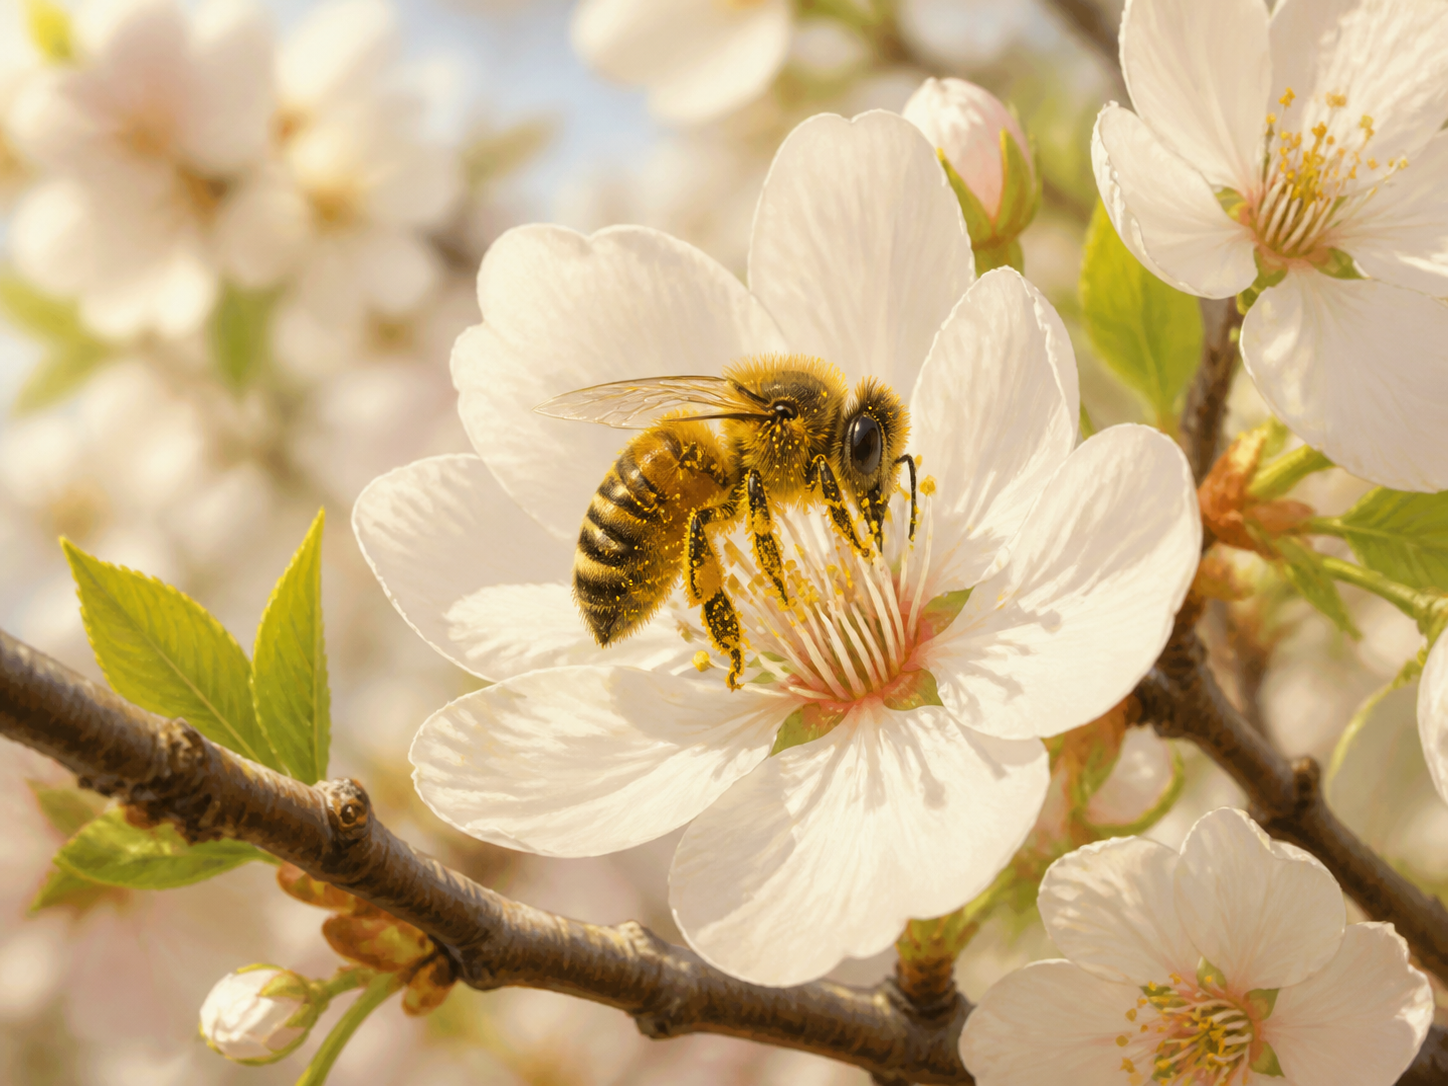
\includegraphics[width=0.58\linewidth]{images/book1/ai/g3-flowers-bee.png}

{\small Bestuiving in volle gang: een bij diep in een kersenbloesem,
bestoven met het \omterm{def:g3:flowers-fruits-seeds:parts}{stuifmeel} dat ze bij de volgende \omterm{def:g3:flowers-fruits-seeds:parts}{bloem} zal bezorgen.}
\end{omfigure}

\section{Vrucht of geen vrucht?}

\begin{method}[De zaadtest]\label{met:g3:flowers-fruits-seeds:test}
Om te beslissen of iets van de groenteboer een \omterm{prop:g3:flowers-fruits-seeds:transform}{vrucht} is in de zin van
de bioloog:
\begin{enumerate}
  \item snijd het open;
  \item zoek naar \omterm{prop:g3:flowers-fruits-seeds:transform}{zaden} (of een pit, dat is een \omterm{def:g2:from-seed-to-plant:seed}{zaad} in een harde schil);
  \item \omterm{prop:g3:flowers-fruits-seeds:transform}{zaden} erin --- het is uit de \omterm{def:g3:flowers-fruits-seeds:parts}{stamper} van een \omterm{def:g3:flowers-fruits-seeds:parts}{bloem} gegroeid: een
        \omterm{prop:g3:flowers-fruits-seeds:transform}{vrucht}. Nergens \omterm{prop:g3:flowers-fruits-seeds:transform}{zaden} --- het is een ander deel van de \omterm{def:g1:plants-around-us:plant}{plant}:
        \omterm{def:g1:plants-around-us:parts}{wortel}, \omterm{def:g1:plants-around-us:parts}{stengel} of \omterm{def:g1:plants-around-us:parts}{blad}.
\end{enumerate}
\end{method}

\begin{example}[Verrassingen bij de groenteboer]\label{ex:g3:flowers-fruits-seeds:surprise}
De zaadtest levert verrassingen op. Tomaat: vol \omterm{prop:g3:flowers-fruits-seeds:transform}{zaden} --- een \omterm{prop:g3:flowers-fruits-seeds:transform}{vrucht},
wat de saladeschaal er ook van zegt. Komkommer en courgette: \omterm{prop:g3:flowers-fruits-seeds:transform}{zaden} ---
\omterm{prop:g3:flowers-fruits-seeds:transform}{vruchten}. Sperzieboonpeul: \omterm{prop:g3:flowers-fruits-seeds:transform}{zaden} op een rij --- een \omterm{prop:g3:flowers-fruits-seeds:transform}{vrucht}. \omterm{def:g1:plants-around-us:parts}{Wortel}:
geen \omterm{prop:g3:flowers-fruits-seeds:transform}{zaden} --- een \omterm{def:g1:plants-around-us:parts}{wortel} (\cref{exo:g1:plants-around-us:10} raadde het
al). Sla: geen \omterm{prop:g3:flowers-fruits-seeds:transform}{zaden} --- \omterm{def:g1:plants-around-us:parts}{bladeren}. Aardappel: geen \omterm{prop:g3:flowers-fruits-seeds:transform}{zaden} --- een
opgezwollen ondergrondse \omterm{def:g1:plants-around-us:parts}{stengel}.
\end{example}

\begin{remark}[Keukenwoorden, wetenschapswoorden]\label{rem:g3:flowers-fruits-seeds:words}
In de keuken betekent ``fruit'' zoet en ``groente'' hartig --- handig
om het toetje te plannen, nutteloos voor de \omterm{def:g1:living-or-not:living}{biologie}. Het woord van de
bioloog volgt de zaadtest. Allebei de woordenschatten zijn prima, zolang
je weet welke je spreekt.
\end{remark}

\section{Oefeningen}

\begin{exercise}[$\star$]\label{exo:g3:flowers-fruits-seeds:1}
Noem de delen van een \omterm{def:g3:flowers-fruits-seeds:parts}{bloem} van buiten naar binnen, met de taak van elk deel.
\end{exercise}

\begin{exercise}[$\star$]\label{exo:g3:flowers-fruits-seeds:2}
Wat is \omterm{def:g3:flowers-fruits-seeds:parts}{stuifmeel}, en waar zit het? Wat is bestuiving?
\end{exercise}

\begin{exercise}[$\star$]\label{exo:g3:flowers-fruits-seeds:3}
Wat wordt er na de bestuiving van: (a) de \omterm{def:g3:flowers-fruits-seeds:parts}{kroonbladen}? (b) de \omterm{def:g3:flowers-fruits-seeds:parts}{stamper}?
(c) de toekomstige \omterm{prop:g3:flowers-fruits-seeds:transform}{zaden} erin?
\end{exercise}

\begin{exercise}[$\star$]\label{exo:g3:flowers-fruits-seeds:4}
Vertel het verhaal van één kers na, van witte bloesem tot rode \omterm{prop:g3:flowers-fruits-seeds:transform}{vrucht},
in drie gedateerde stappen.
\end{exercise}

\begin{exercise}[$\star$]\label{exo:g3:flowers-fruits-seeds:5}
Waarom verwelkomen kersentelers bijenkasten in de boomgaard?
\end{exercise}

\begin{exercise}[$\star$]\label{exo:g3:flowers-fruits-seeds:6}
Noem de zaadtest, en pas hem toe op de tomaat en de \omterm{def:g1:plants-around-us:parts}{wortel}.
\end{exercise}

\begin{exercise}[$\star$]\label{exo:g3:flowers-fruits-seeds:7}
\omterm{prop:g3:flowers-fruits-seeds:transform}{Vrucht} of niet, volgens de zaadtest: de komkommer, de sla, de
sperzieboonpeul, de aardappel?
\end{exercise}

\begin{exercise}[$\star$]\label{exo:g3:flowers-fruits-seeds:8}
Probeer het: snijd thuis drie dingen uit de keuken open en laat de
zaadtest erop los. Welke verraste je?
\end{exercise}

\begin{exercise}[$\star\star$]\label{exo:g3:flowers-fruits-seeds:9}
Een late nachtvorst doodt in april alle bloesem aan de pruimenboom. Wat
wordt de oogst in juni, en waarom? Gebruik
\cref{prop:g3:flowers-fruits-seeds:transform}.
\end{exercise}

\begin{exercise}[$\star\star$]\label{exo:g3:flowers-fruits-seeds:10}
``De appel groeit zodat wij iets lekkers te eten hebben.'' Waar dient
de appel echt voor, vanuit het oogpunt van de appelboom? Wat ligt er in
zijn klokhuis, en wat zou elk daarvan kunnen worden? (Denk aan
\cref{ch:g2:from-seed-to-plant}.)
\end{exercise}
